\subsection{Backpropagation}

\begin{frame}
\frametitle{Notation}

\begin{figure}
	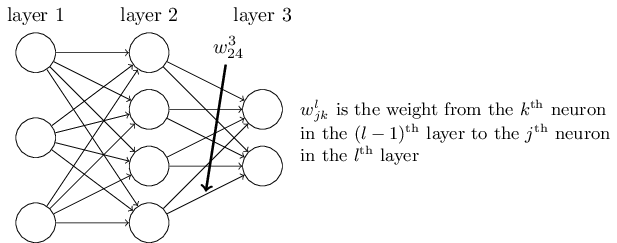
\includegraphics[width=\linewidth]{./aktuelleEntwicklung/backpropagation/img/weight_notation}
\end{figure}

\note[item]{l: Exponent, steht für die Schicht}
\note[item]{l - 1, weil man stets von hinten nach vorne schaut}
\note[item]{Eingabe wird auch als eigene Schicht verstanden}
\note[item]{j: Index Zielneuron}
\note[item]{k: Index Startneuron}

\end{frame}

\begin{frame}
\frametitle{Notation}

\begin{figure}
	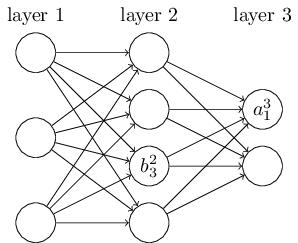
\includegraphics[width=.6\linewidth]{./aktuelleEntwicklung/backpropagation/img/biasAct_notation}
	
\note[item]{Ähnlich zu Gewichtsnotation}
\note[item]{l bezieht sich hierbei jedoch auf aktuelle Schicht}
\note[item]{j wie gehabt Index in Schicht}
\note[item]{Notation gilt auch für Aktivierung a}

\end{figure}

\begin{columns}

\column{.5\textwidth}
\begin{align*}
a^{l}_j = \sigma\left( \sum_k w^{l}_{jk} a^{l-1}_k + b^l_j \right) \Rightarrow 
\quad
\!
\begin{aligned}
a^l & = \sigma(z^l) \\
z^l & = w^l a^{l-1}+b^l \\
\end{aligned}
\end{align*}

\note[item]{Wichtig: $\sigma$ bezieht sich auf Vektor $\Rightarrow$ Vektorielle Funktion}
\note[item]{Jede Komponente einzeln mit $\sigma$ verarbeitet}
\note[item]{Abstraktion vom Ausgabewert vor der Aktivierungsfkt. hilft später beim Ableiten}

\hspace{10mm}

\end{columns}

\end{frame}



\begin{frame}
\frametitle{Backpropagation}

\begin{itemize}
\item{Kostenfunktion soll minimiert werden}
\item{Ziel: Optimale Gewichte und Schwellwerte finden}
\end{itemize}

\begin{itemize}
\item Grobe Vorgehensweise: Iterativer Prozess

\begin{itemize}	
	\item Fehlervektor der letzten Schicht berechnen
	\item Fehler schichtweise zum Eingabelayer zurückführen
	\item Parameter schichtweise nach Gradienten angleichen
\end{itemize}

\end{itemize}


\note[item]{Kostenfunktion wie bei Gradientenabstieg / Adeline}
\note[item]{Unterschied: Hier mehrschichtiges Netz}
\note[item]{1970er entwickelt, 1986 von Rummelhart, Hilten und Williams in Paper bekannt gemacht}
\note[item]{Gradientenabstieg grob erläutert, ausgeblieben - Anwendung im mehrschichtigen Netz und mehrdimensionale Kostenfunktion}

\note[item]{Fehlervektor der letzten Schicht berechnen}
\note[item]{Fehler schichtweise zum Eingabelayer zurückführen}
\note[item]{Parameter schichtweise nach Gradienten angleichen}
\end{frame}



\begin{frame}
\frametitle{Aufbau}

%\begin{figure}[!htb]
%	\centering

%\Tree [.C y [.$a^{l+1}_j$ {\bf b} c ] d ]

	
\Tree [.C y [.$a^{l+1}_j$ [ .$z^{l+1}_j$ [ $w^l_j$ [ .$a^l_j$ [ .$z^l_j$ $w^l_j$ $a^{l-1}_j$ $b^{l-1}_j$ ] ] $b^{l-1}_j$ ] ] ] ]
%	\caption [Baumdarstellung]{Baumdarstellung - Zusammenhang der Gewichte, Aktivierungen und Schwellwerte \cite{3b1b}}
%	\label{fig:tree}
%\end{figure}
\end{frame}



\begin{frame}
\frametitle{Fundamentale Gleichungen - 1} 

\begin{itemize}
\item Fehlervektor der letzten Schicht berechnen: \inlineeq{\delta^L = \nabla_a C \odot \sigma'(z^L)}
\end{itemize}

\begin{columns}

\column{0.5\textwidth}
\myeq{
\delta^L_j & = \frac{\partial C}{\partial z^L_j} \\
 & = \sum_k \frac{\partial C}{\partial a^L_k} \frac{\partial a^L_k}{\partial z^L_j}
}

\column{0.5\textwidth}





\begin{block}{Anmerkung: Kettenregel}
\myeq{\frac{d}{{dx}}\left[ {f\left( u \right)} \right] = \frac{d}{{du}}\left[ {f\left( u \right)} \right]\frac{{du}}{{dx}}}
\end{block}

\end{columns}


\note[item]{Großes L immer für Ausgabeschicht}

\end{frame}

